%%% TITLE AND AUTHORS %%%%%%%%%%%%%%%%%%%%%%%%%%%%%%%%%%%%%%%%%%%%%%%%%%%%%%%%%
\title[Data from external sources]{
    Extracting existing data from external sources \\
}
\author[]{Szymon Talaga and Mikołaj Biesaga} % Your name
\institute[ISS UW]{
    The Robert Zajonc Institute for Social Studies \\ University of Warsaw \\
    \medskip
    \textcolor{blue}{\href{mailto:stalaga@uw.edu.pl}{stalaga@uw.edu.pl}} \\
    \textcolor{blue}{\href{mailto:m.biesaga@uw.edu.pl}{m.biesaga@uw.edu.pl}}
}
\date{30 October 2019} % Date, can be changed to a custom date

%%% SLIDES %%%%%%%%%%%%%%%%%%%%%%%%%%%%%%%%%%%%%%%%%%%%%%%%%%%%%%%%%%%%%%%%%%%%
\frame{\titlepage}

\section[API]{Web Application Programming Interface}

\begin{frame}
    \only<+>{
        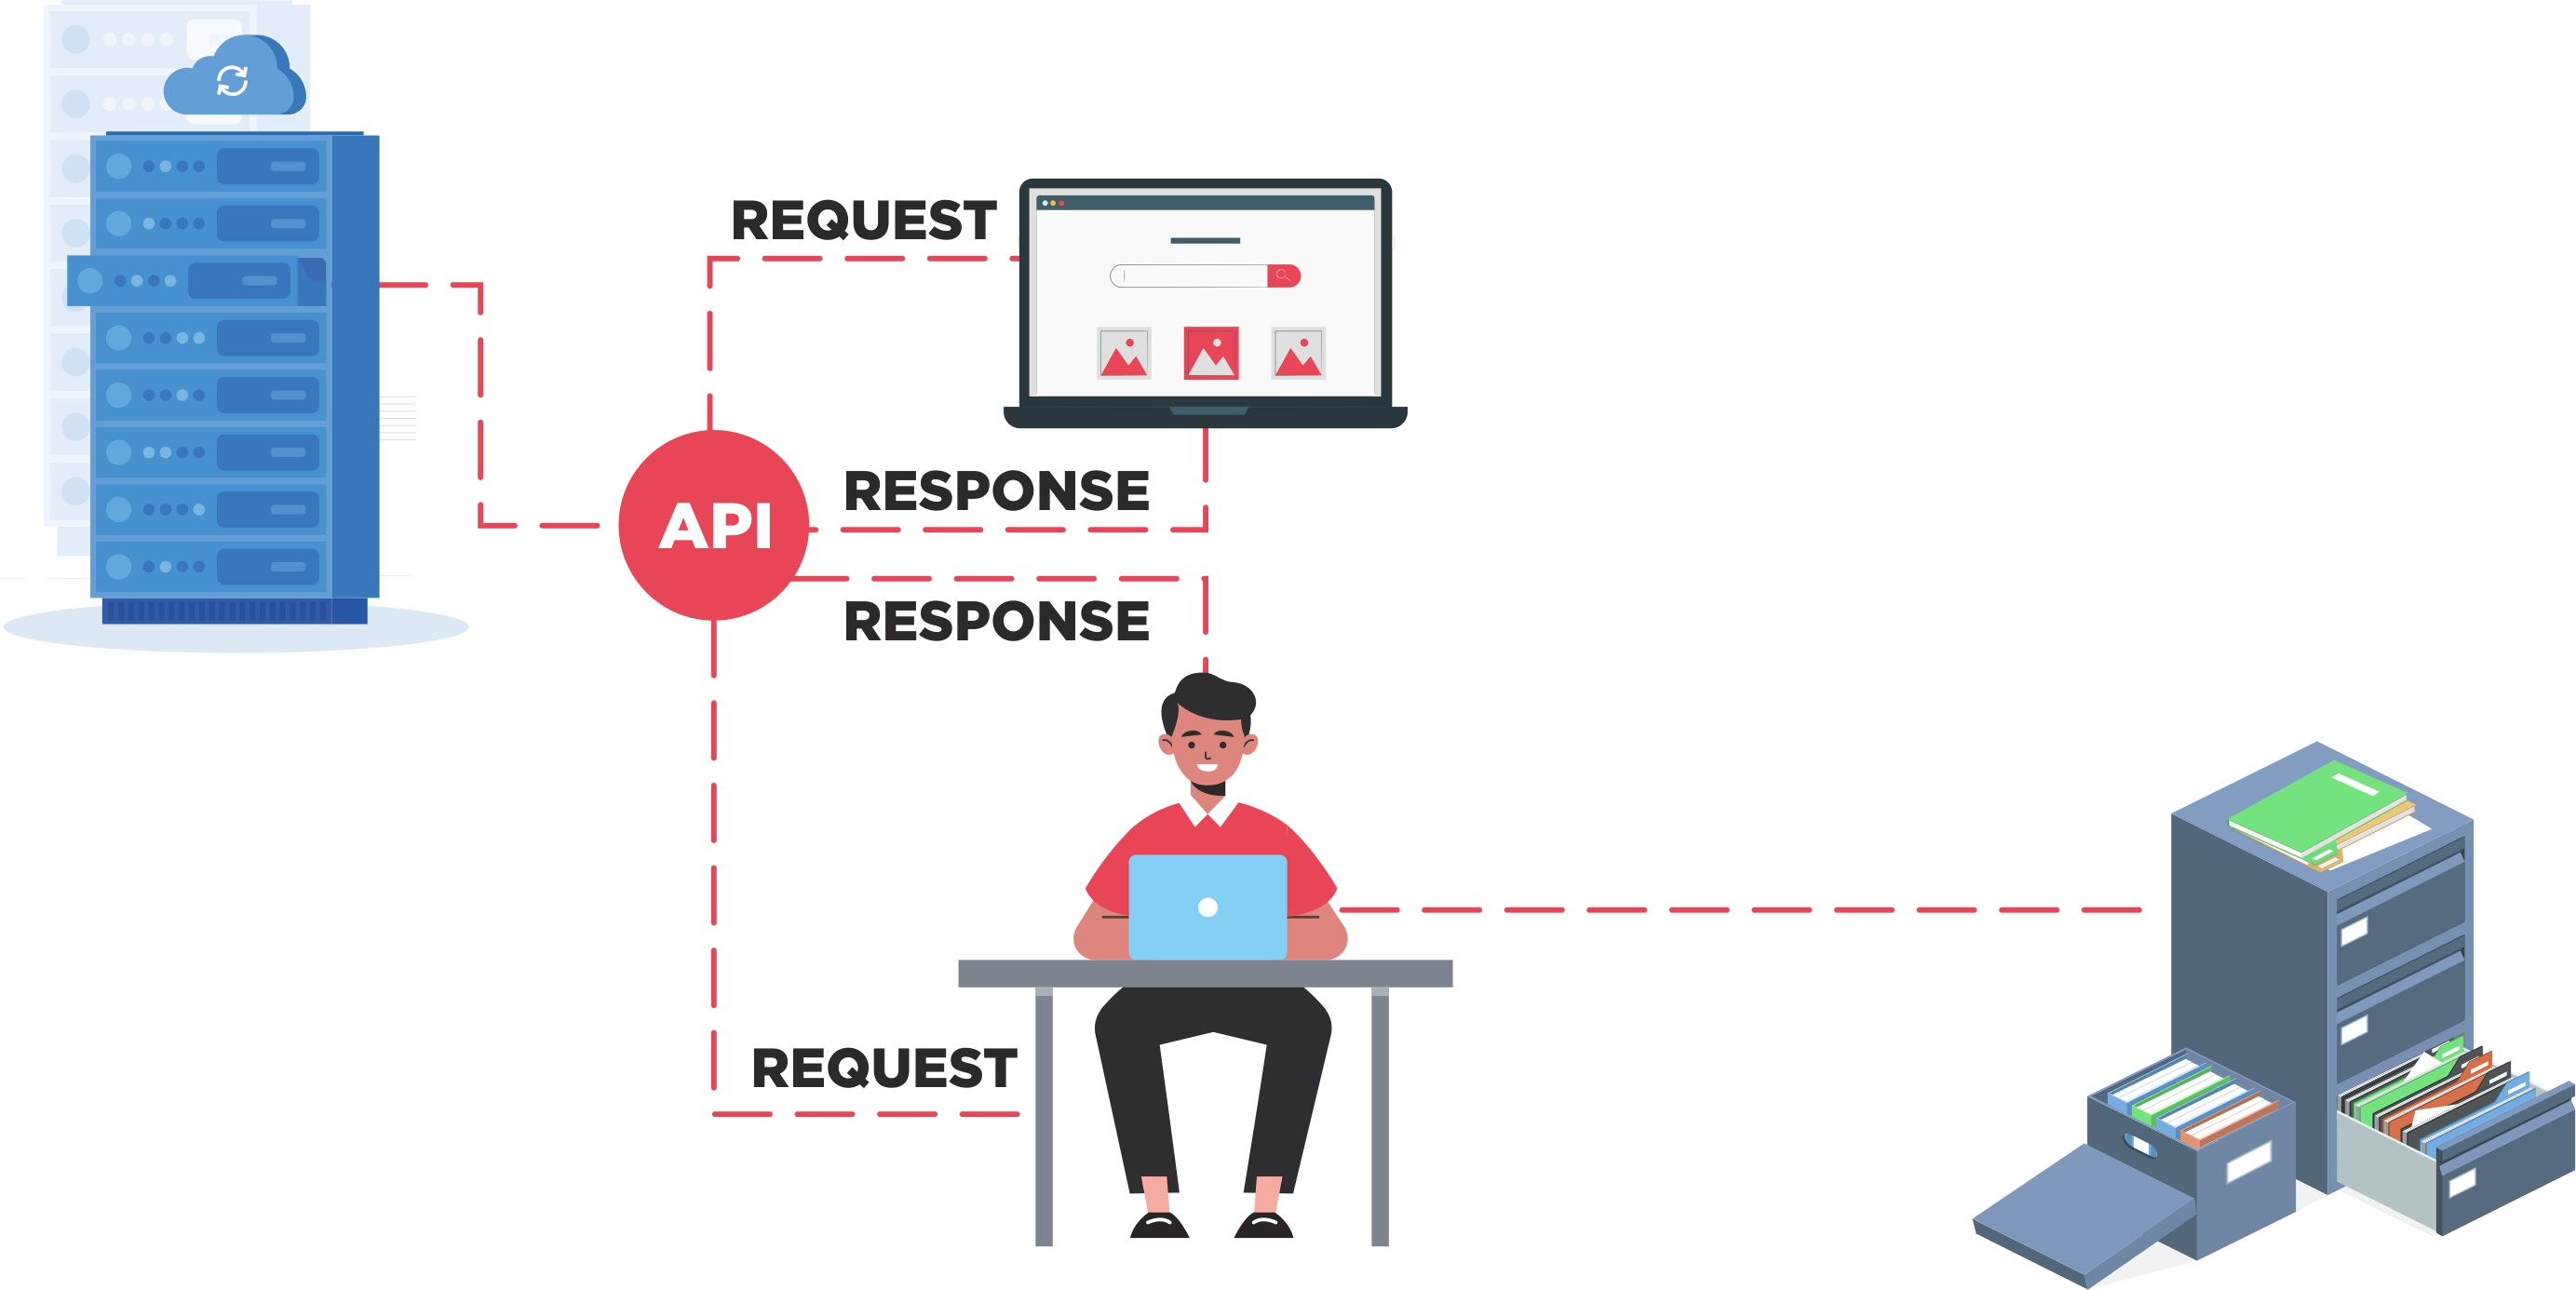
\includegraphics[width = \framewidth]{png/api.jpg}
    }
    \only<+>{
        \begin{definition}
            \emph{Aplication Programming Interface} is a communication protocol between a client and a server intended to simplify the building of client-side software. In other words, it is a contract between the client and the server which defines the format of possible requests and format of the response (i.e. format of the data).
        \end{definition}
    }
\end{frame}


\subsection{HTML}
\begin{frame}
    \only<+>{
        \frametitle{Web browsing}
        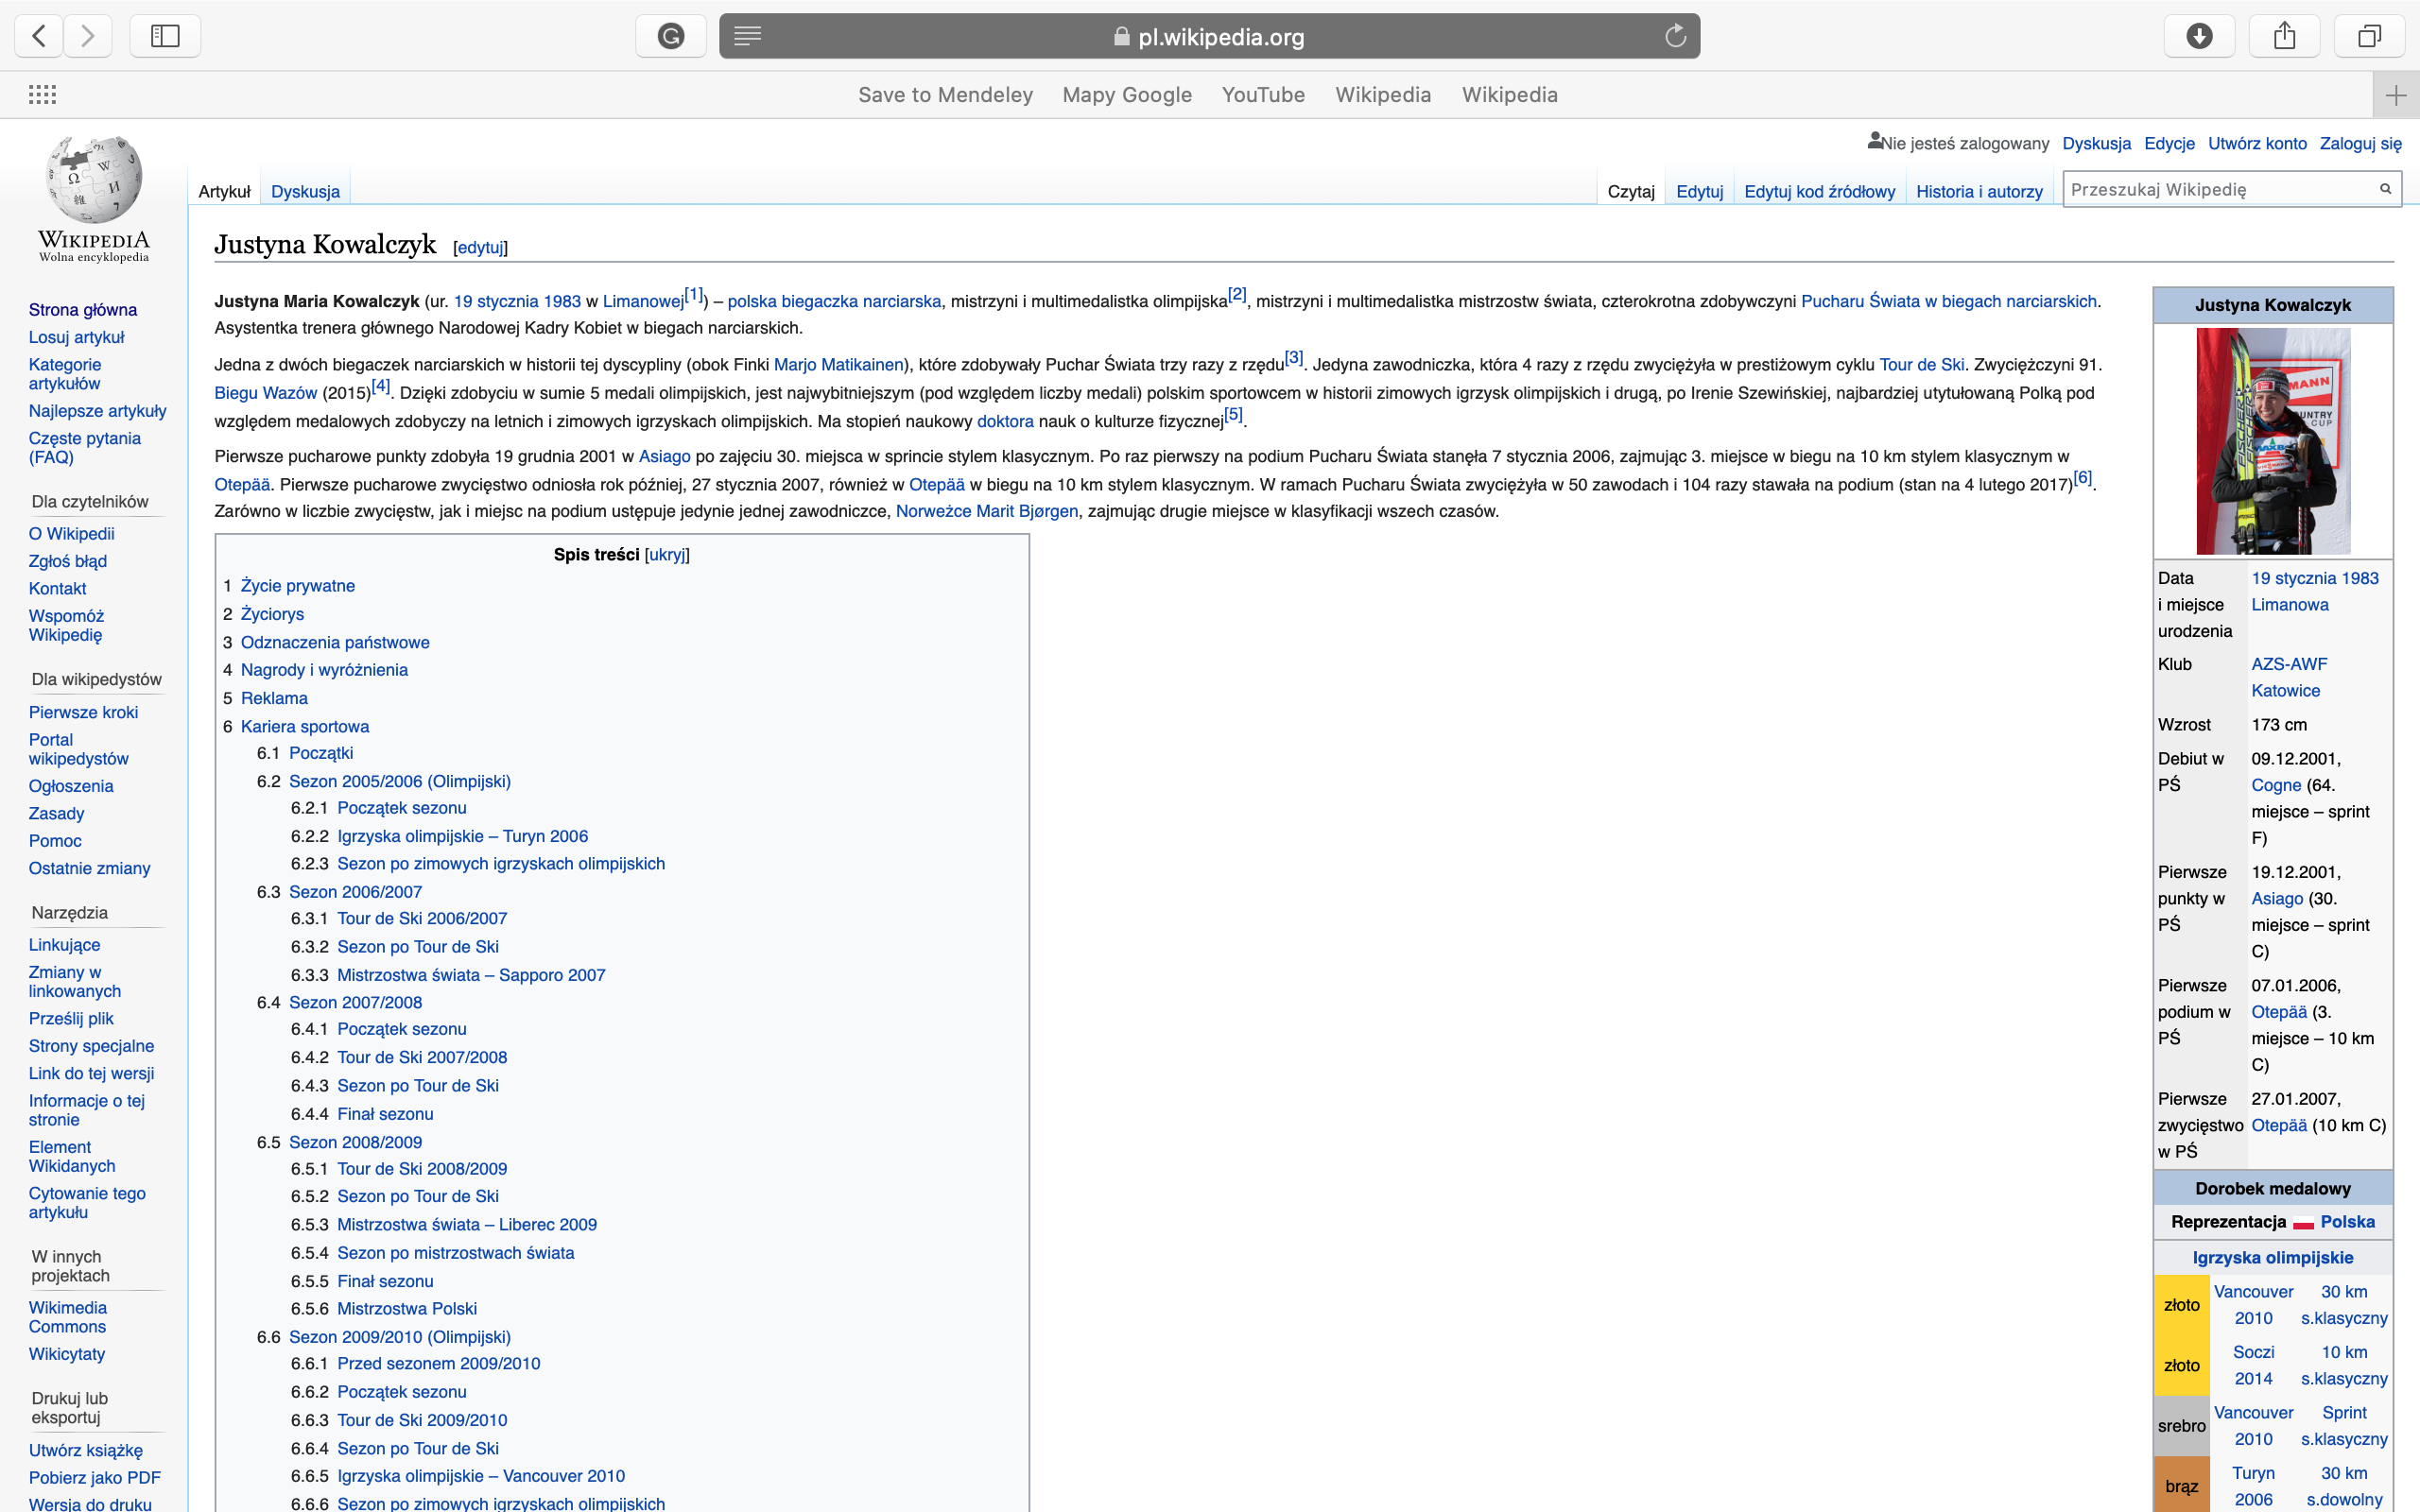
\includegraphics[width = \framewidth]{png/webpage.png}
    }
    \only<+>{
        \frametitle{Web browsing}
        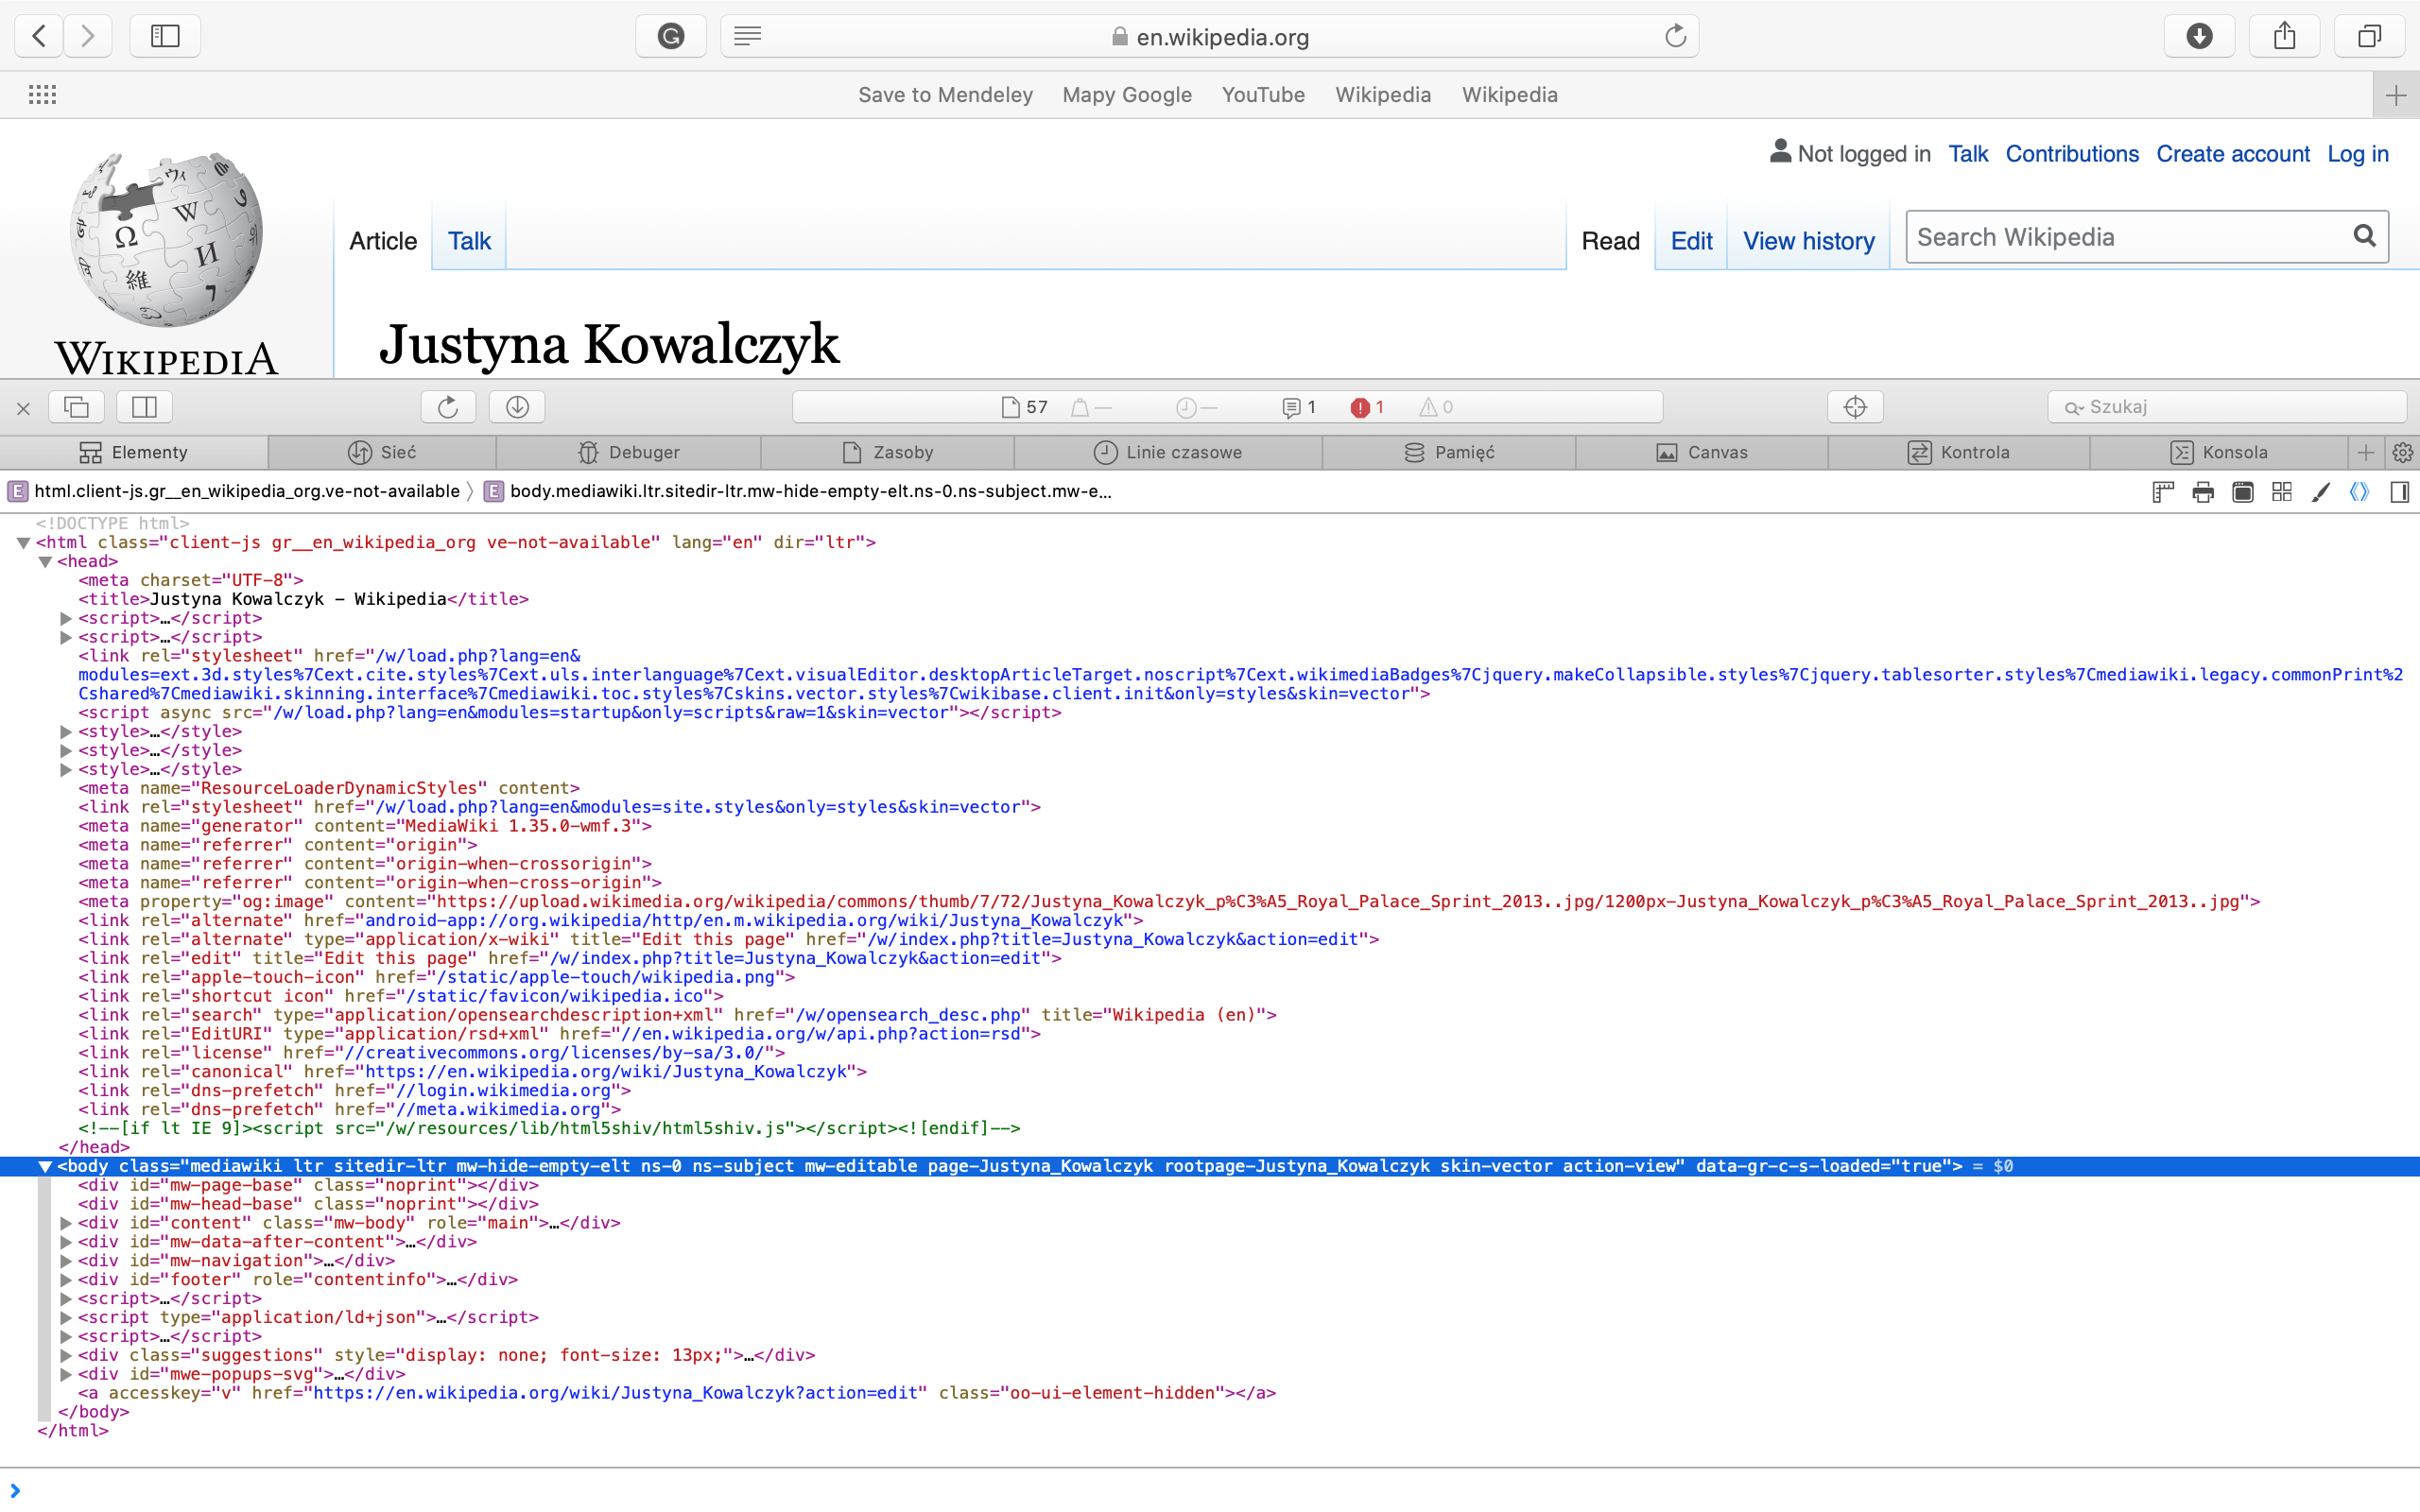
\includegraphics[width = \framewidth]{png/webpage_html.png}
    }
    \only<+>{
        \frametitle{Hypertext Markup Language}
        \begin{definition}
            \emph{Hypertext Markup Language} (HTML) is the standard markup language for documents designed to be displayed in a web browser. It can be assisted by technologies such as Cascading Style Sheets (CSS) and scripting languages such as JavaScript.
            Web browsers receive HTML documents from a web server or local storage and render the documents into multimedia web pages. HTML describes the structure of a web page semantically and originally included cues for the appearance of the document.
        \end{definition}
    }
\end{frame}

\begin{frame}[fragile]
    \frametitle{HTML example}
    \begin{minted}[escapeinside=||,mathescape=true]{html}
<!DOCTYPE html>
<html>
    <head>
        <title>
            Justyna Kowalczyk fandom
        </title>
    </head>
    <body>
        <p>
            Justyna Kowalczyk |<|3
        </p>
    </body>
</html>
    \end{minted}
\end{frame}

\subsection{CSS}

\begin{frame}
        \frametitle{Cascading Style Sheets}
        \begin{definition}
            \emph{Cascading Style Sheets} (CSS) is a style sheet language used for describing the presentation of a document written in a markup language like HTML.
        \end{definition}
\end{frame}

\begin{frame}[fragile]
    \frametitle{CSS}
    \begin{minted}[escapeinside=||,mathescape=true]{html}
<!DOCTYPE html>
<html>
    <head>
        <title>
            Justyna Kowalczyk fandom
        </title>
        <style>
            .person {
                color: red;
            }
        </style>
    </head>
    <body>
        <p class="person">
            Justyna Kowalczyk |<|3
        </p>
    </body>
</html>
    \end{minted}
\end{frame}

\begin{frame}
    \only<+>{
        \frametitle{Web browsing without CSS}
        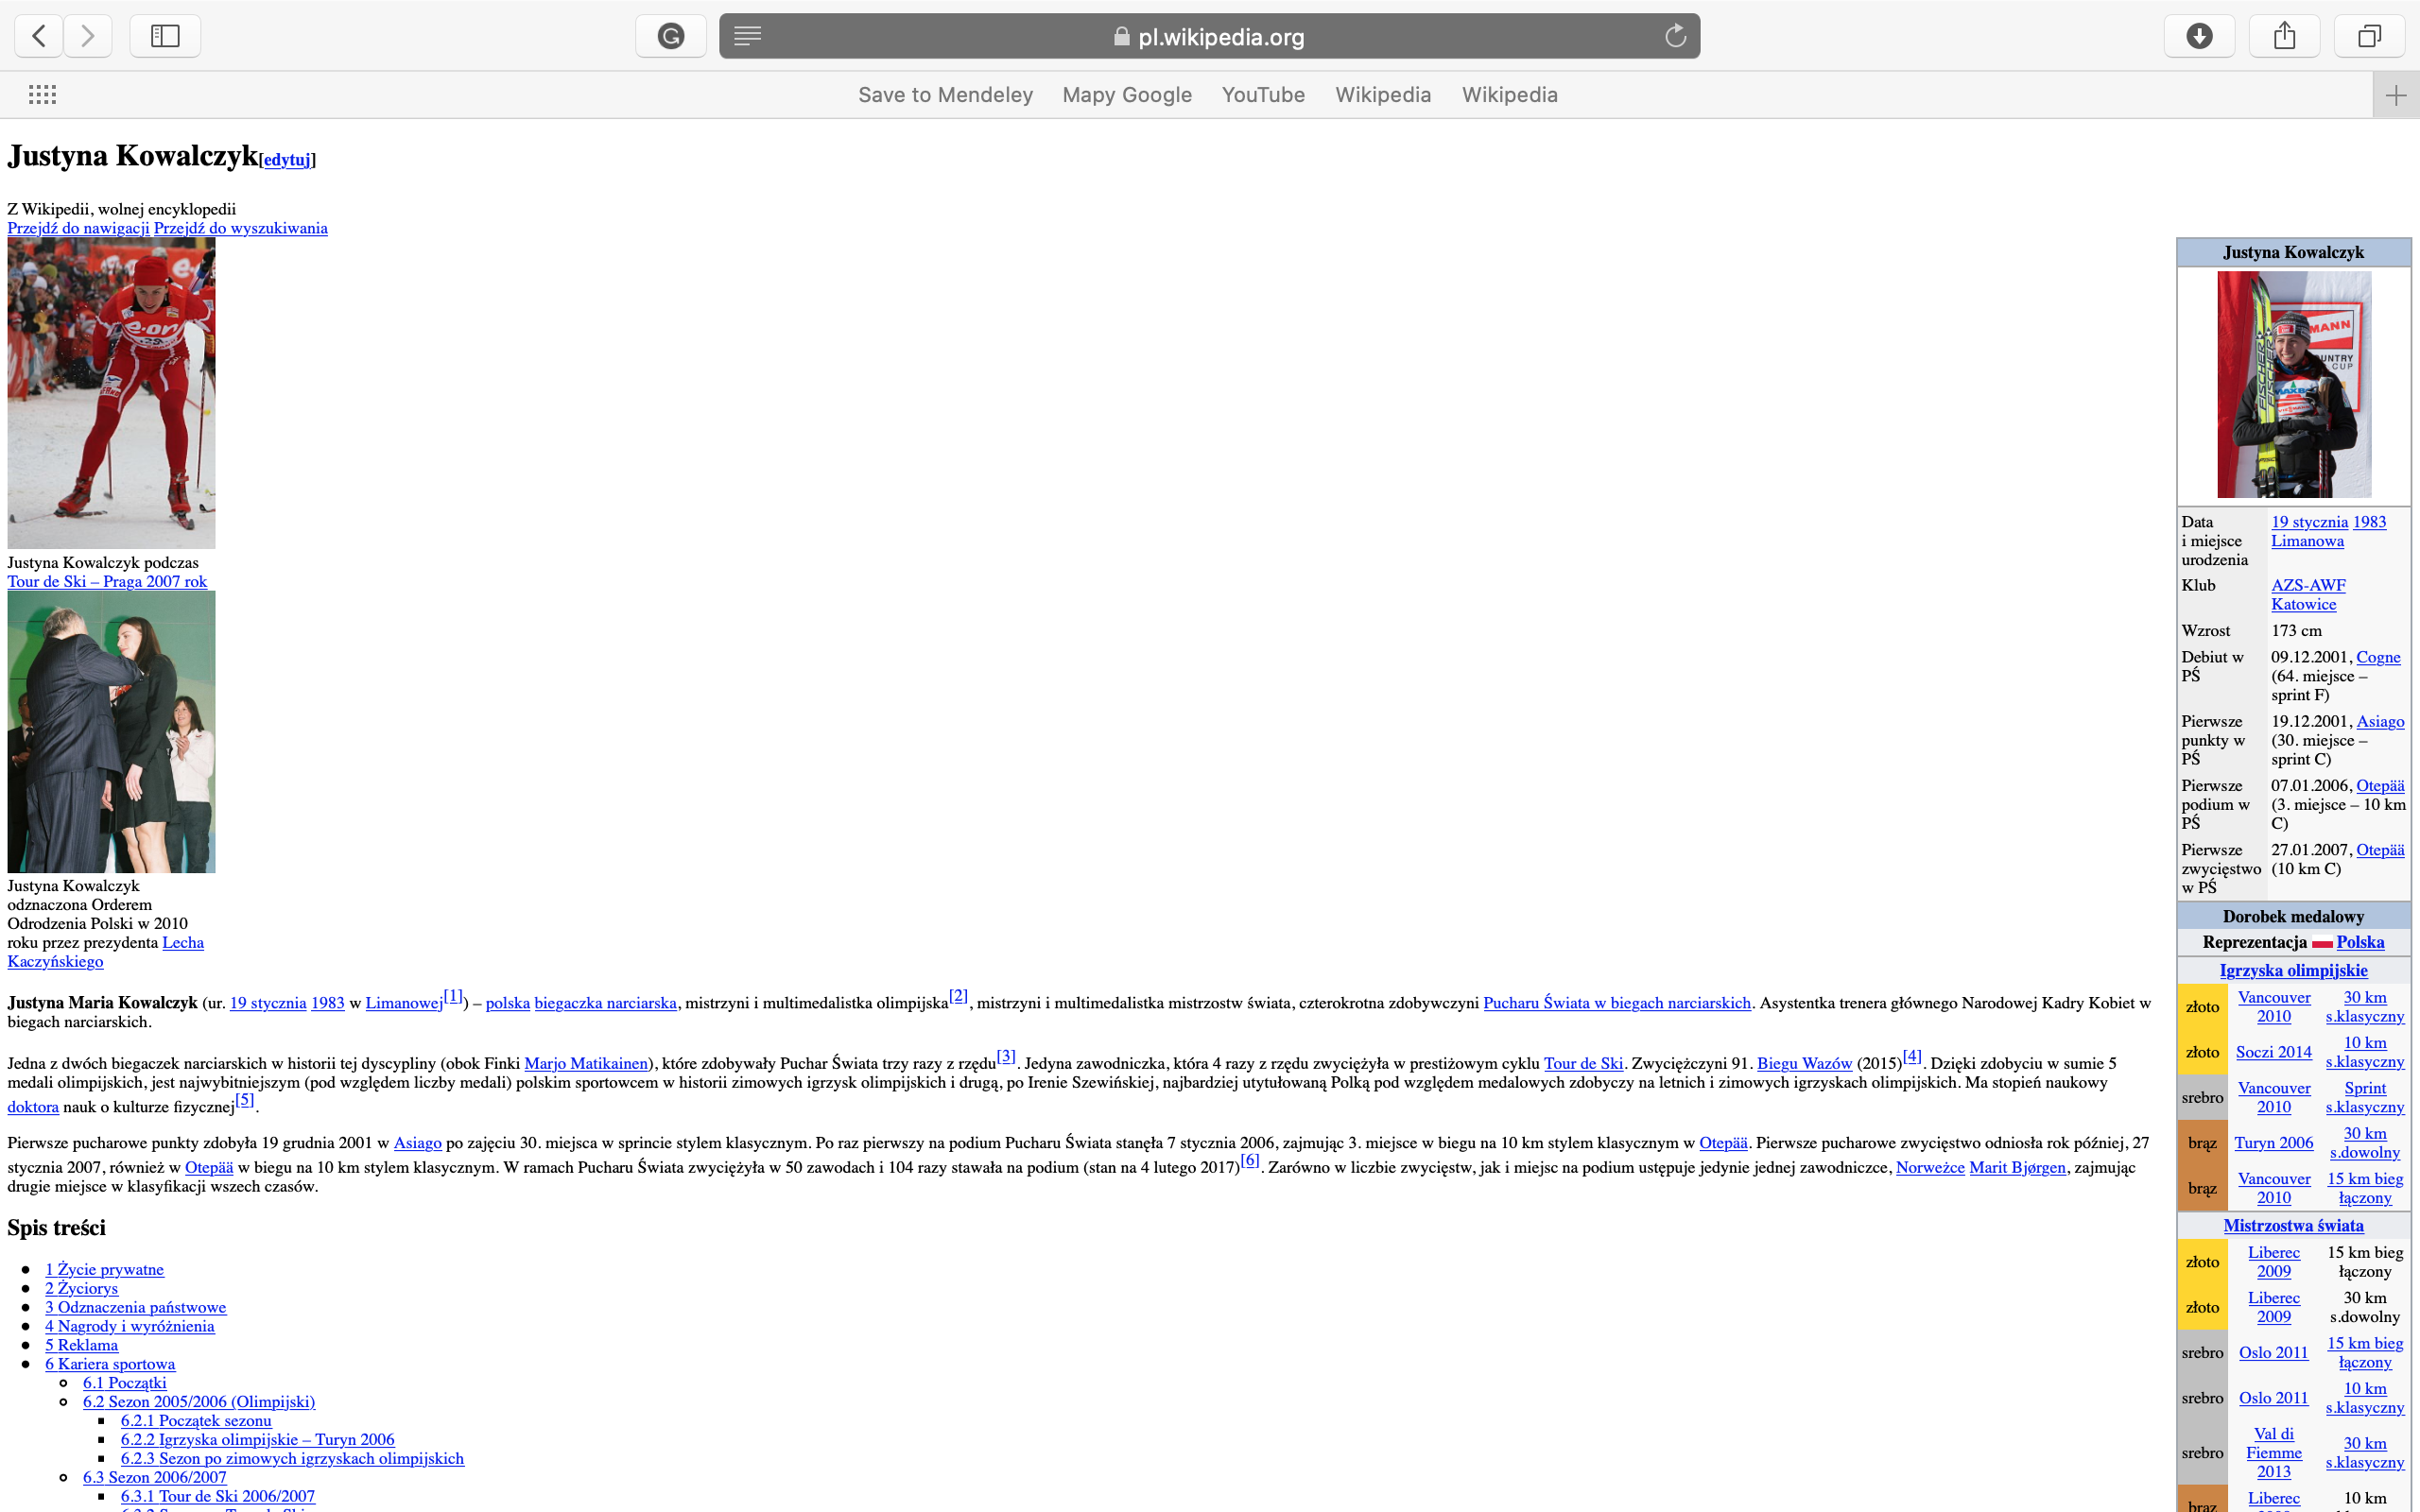
\includegraphics[width = \framewidth]{png/webpage_nostyle.png}
    }
    \only<+>{
        \frametitle{Web browsing without CSS}
        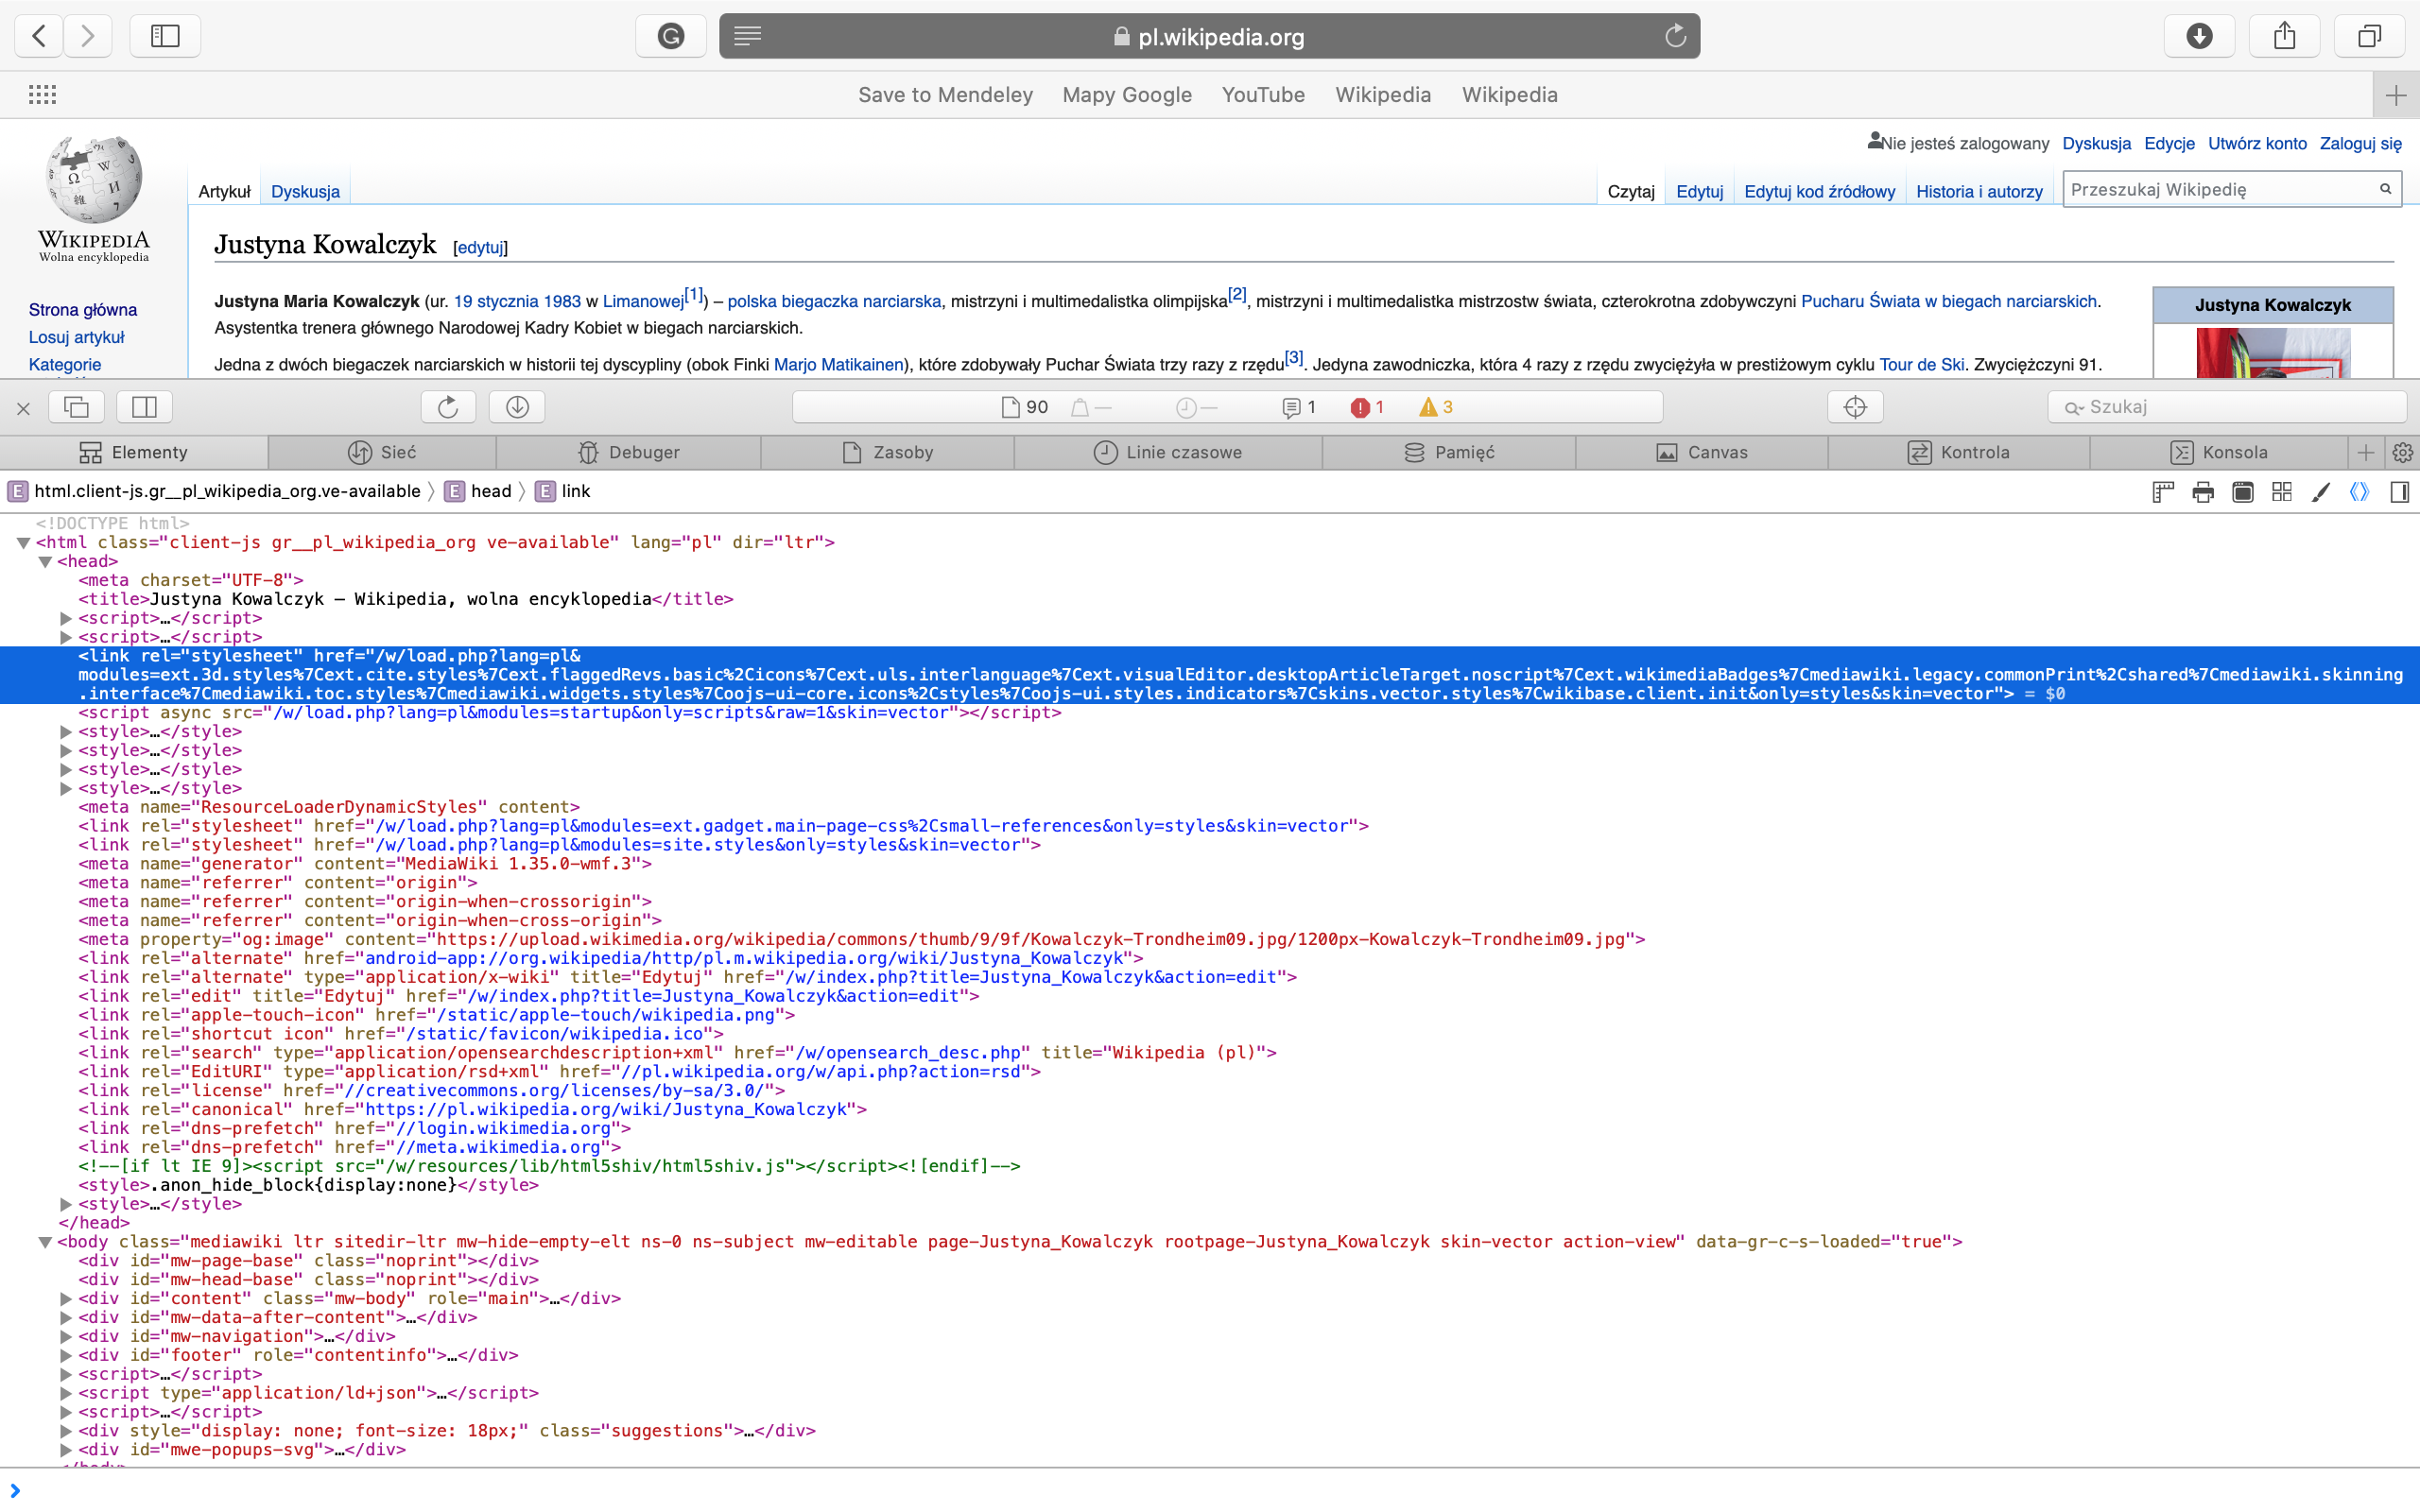
\includegraphics[width = \framewidth]{png/webpage_css.png}
    }
\end{frame}

\begin{frame}
    \only<+>{
        \frametitle{Types of Web APIs}
        \setbeamercovered{transparent}
        \begin{itemize}
            \item<0> SOAP (Simple Object Access Protocol)
            \item<0> RPC (Remote Procedure Call)
            \item REST (REpresentational State Transfer)
        \end{itemize}
    }
\end{frame}
\subsection{REST}
\begin{frame}
    \only<1>{
        \frametitle{REST (REpresentational State Transfer)}
        \begin{definition}
            The \emph{Representational State Transfer} (REST) is an abstraction of the architectural elements within a distributed hypermedia system. It ignores the details of component implementation and protocol syntax to focus on the roles of components, the constraints upon their interaction with other components, and their interpretation of significant data elements. It encompasses the fundamental constraints upon components, connectors, and data that define the basis of the Web architecture, and thus the essence of its behavior as a network-based application.
        \end{definition}
    }
    \only<2,4,6,8,17,19>{
        \frametitle{REST constraints}
        \begin{enumerate}
            \item<2-> Client-Server
            \item<4-> Stateless
            \item<6-> Cache
            \item<8-> Uniform Interface
            \item<17-> Layered System
            \item<19-> Code-On-Demand*
        \end{enumerate}
    }
    \only<3>{
        \frametitle{Clinet-Server}
        Client and Server are \alert{independent}. They must be able to evolve separately without any dependency on each other. In other words, the application (client) should work regardless of changes on the server-side and the other way around.
    }
    \only<5>{
        \frametitle{Stateless}
        Each request sent by the client to the server must contain \alert{all of the information necessary to understand the request}, and cannot take advantage of any stored context on the server.
    }
    \only<7>{
        \frametitle{Cache}
        Cache constraints require that the data within a response to a request be implicitly or explicitly labeled as cacheable or non-cacheable. If a response is cacheable, then \alert{a client cache is given the right to reuse that response data for later}, equivalent requests.
    }
    \only<9,11,13,15>{
        \frametitle{Uniform Interface}
        To obtain a uniform interface, multiple architectural constraints are needed to guide the behavior of components. REST is defined by four interface constraints:
        \begin{enumerate}
            \item<9-> Resource-Based
            \item<11-> Manipulation of Resources Through Representations
            \item<13-> Self-descriptive Messages
            \item<15-> Hypermedia as the Engine of Application State (HATEOAS)
        \end{enumerate}
    }
    \only<10>{
        \frametitle{Resource-Based}
        The resources themselves are conceptually separate from the representations that are returned to the client. For example, \alert{the server does not send its database}, but rather, some HTML, XML or JSON that represents some database records expressed.
    }
    \only<12>{
        \frametitle{Manipulation of Resources Through Representations}
        When a client \alert{holds a representation of a resource}, including any metadata attached, it \alert{has enough information to modify or delete the resource on the server}, provided it has permission to do so.
    }
    \only<14>{
        \frametitle{Self-descriptive Messages}
        Each message includes \alert{enough information to describe how to process the message}. For example, which parser to invoke. Responses also explicitly indicate their cache-ability.
    }
    \only<16>{
        \frametitle{Hypermedia as the Engine of Application State (HATEOAS)}
        Clients deliver state via \alert{body contents, query-string parameters, request headers and the requested universal resource identifier} (the resource name). Services deliver the state to clients via \alert{body content, response codes, and response headers}. This is technically referred to as hypermedia (or hyperlinks within hypertext).
    }
    \only<18>{
        \frametitle{Layered System}
        A client cannot ordinarily \alert{tell whether it is connected directly to the end server} or an intermediary along the way. Intermediary servers may improve system scalability by enabling load-balancing and by providing shared caches. Layers may also enforce security policies.
    }
    \only<20>{
        \frametitle{Code-On-Demand*}
        Servers are able to send \alert{executable code} to support part of the application on the client-side. In other words, most of the time the server sends a representation of the resources in the form of JSON or XML, but it can also send an executable code.
    }
\end{frame}

\subsection{HTTP}
\begin{frame}
    \only<+>{
        \frametitle{Hypertext Transfer Protocol}
        \begin{definition}
            \emph{Hypertext Transfer Protocol} (HTTP) is is a protocol that allows the fetching of resources, such as HTML documents. It is the foundation of any data exchange on the Web and it is a client-server protocol, which means requests are initiated by the recipient, usually the Web browser. A complete document is reconstructed from the different sub-documents fetched, for instance, text, layout description, images, videos, scripts, and more.
        \end{definition}
    }
    \only<+>{
        \frametitle{HTTP Requests}
        HTTP Requests is typically composed of:
        \begin{itemize}
            \item A start-line (HTTP method, URL/URI, and HTTP version)
            \item An optional set of HTTP headers specifying the request, or describing the body included in the message.
            \item An optional body containing data associated with the request
        \end{itemize}

    }
    \only<+>{
        \frametitle{HTTP Request Methods}
        \begin{itemize}
            \item GET - requests a representation of the specified resource
            \item POST - is used to submit an entity to the specified resource, often causing a change in state or side effects on the server.
            \item PUT - replaces all current representations of the target resource with the request payload.
            \item DELETE - deletes the specified resource.
            \item PATCH - is used to apply partial modifications to a resource.
        \end{itemize}
        \blfootnote{Detailed documentation on \textcolor{blue}{\href{https://developer.mozilla.org/en-US/docs/Web/HTTP/Methods}{Request Methods}}}
    }
\end{frame}

\begin{frame}[fragile]
    \frametitle{HTTP Request}
    \begin{minted}{html}
    GET page/summary/Justyna_Kowalczyk HTTP/1.1
    Host: www.en.mikopedia.org/api/rest_v1/
    Accept: application/json
    User-Agent: m.biesaga@uw.edu.pl
    Body: {}
    \end{minted}
\end{frame}


\begin{frame}
    \only<+>{
        \frametitle{HTTP Response}
        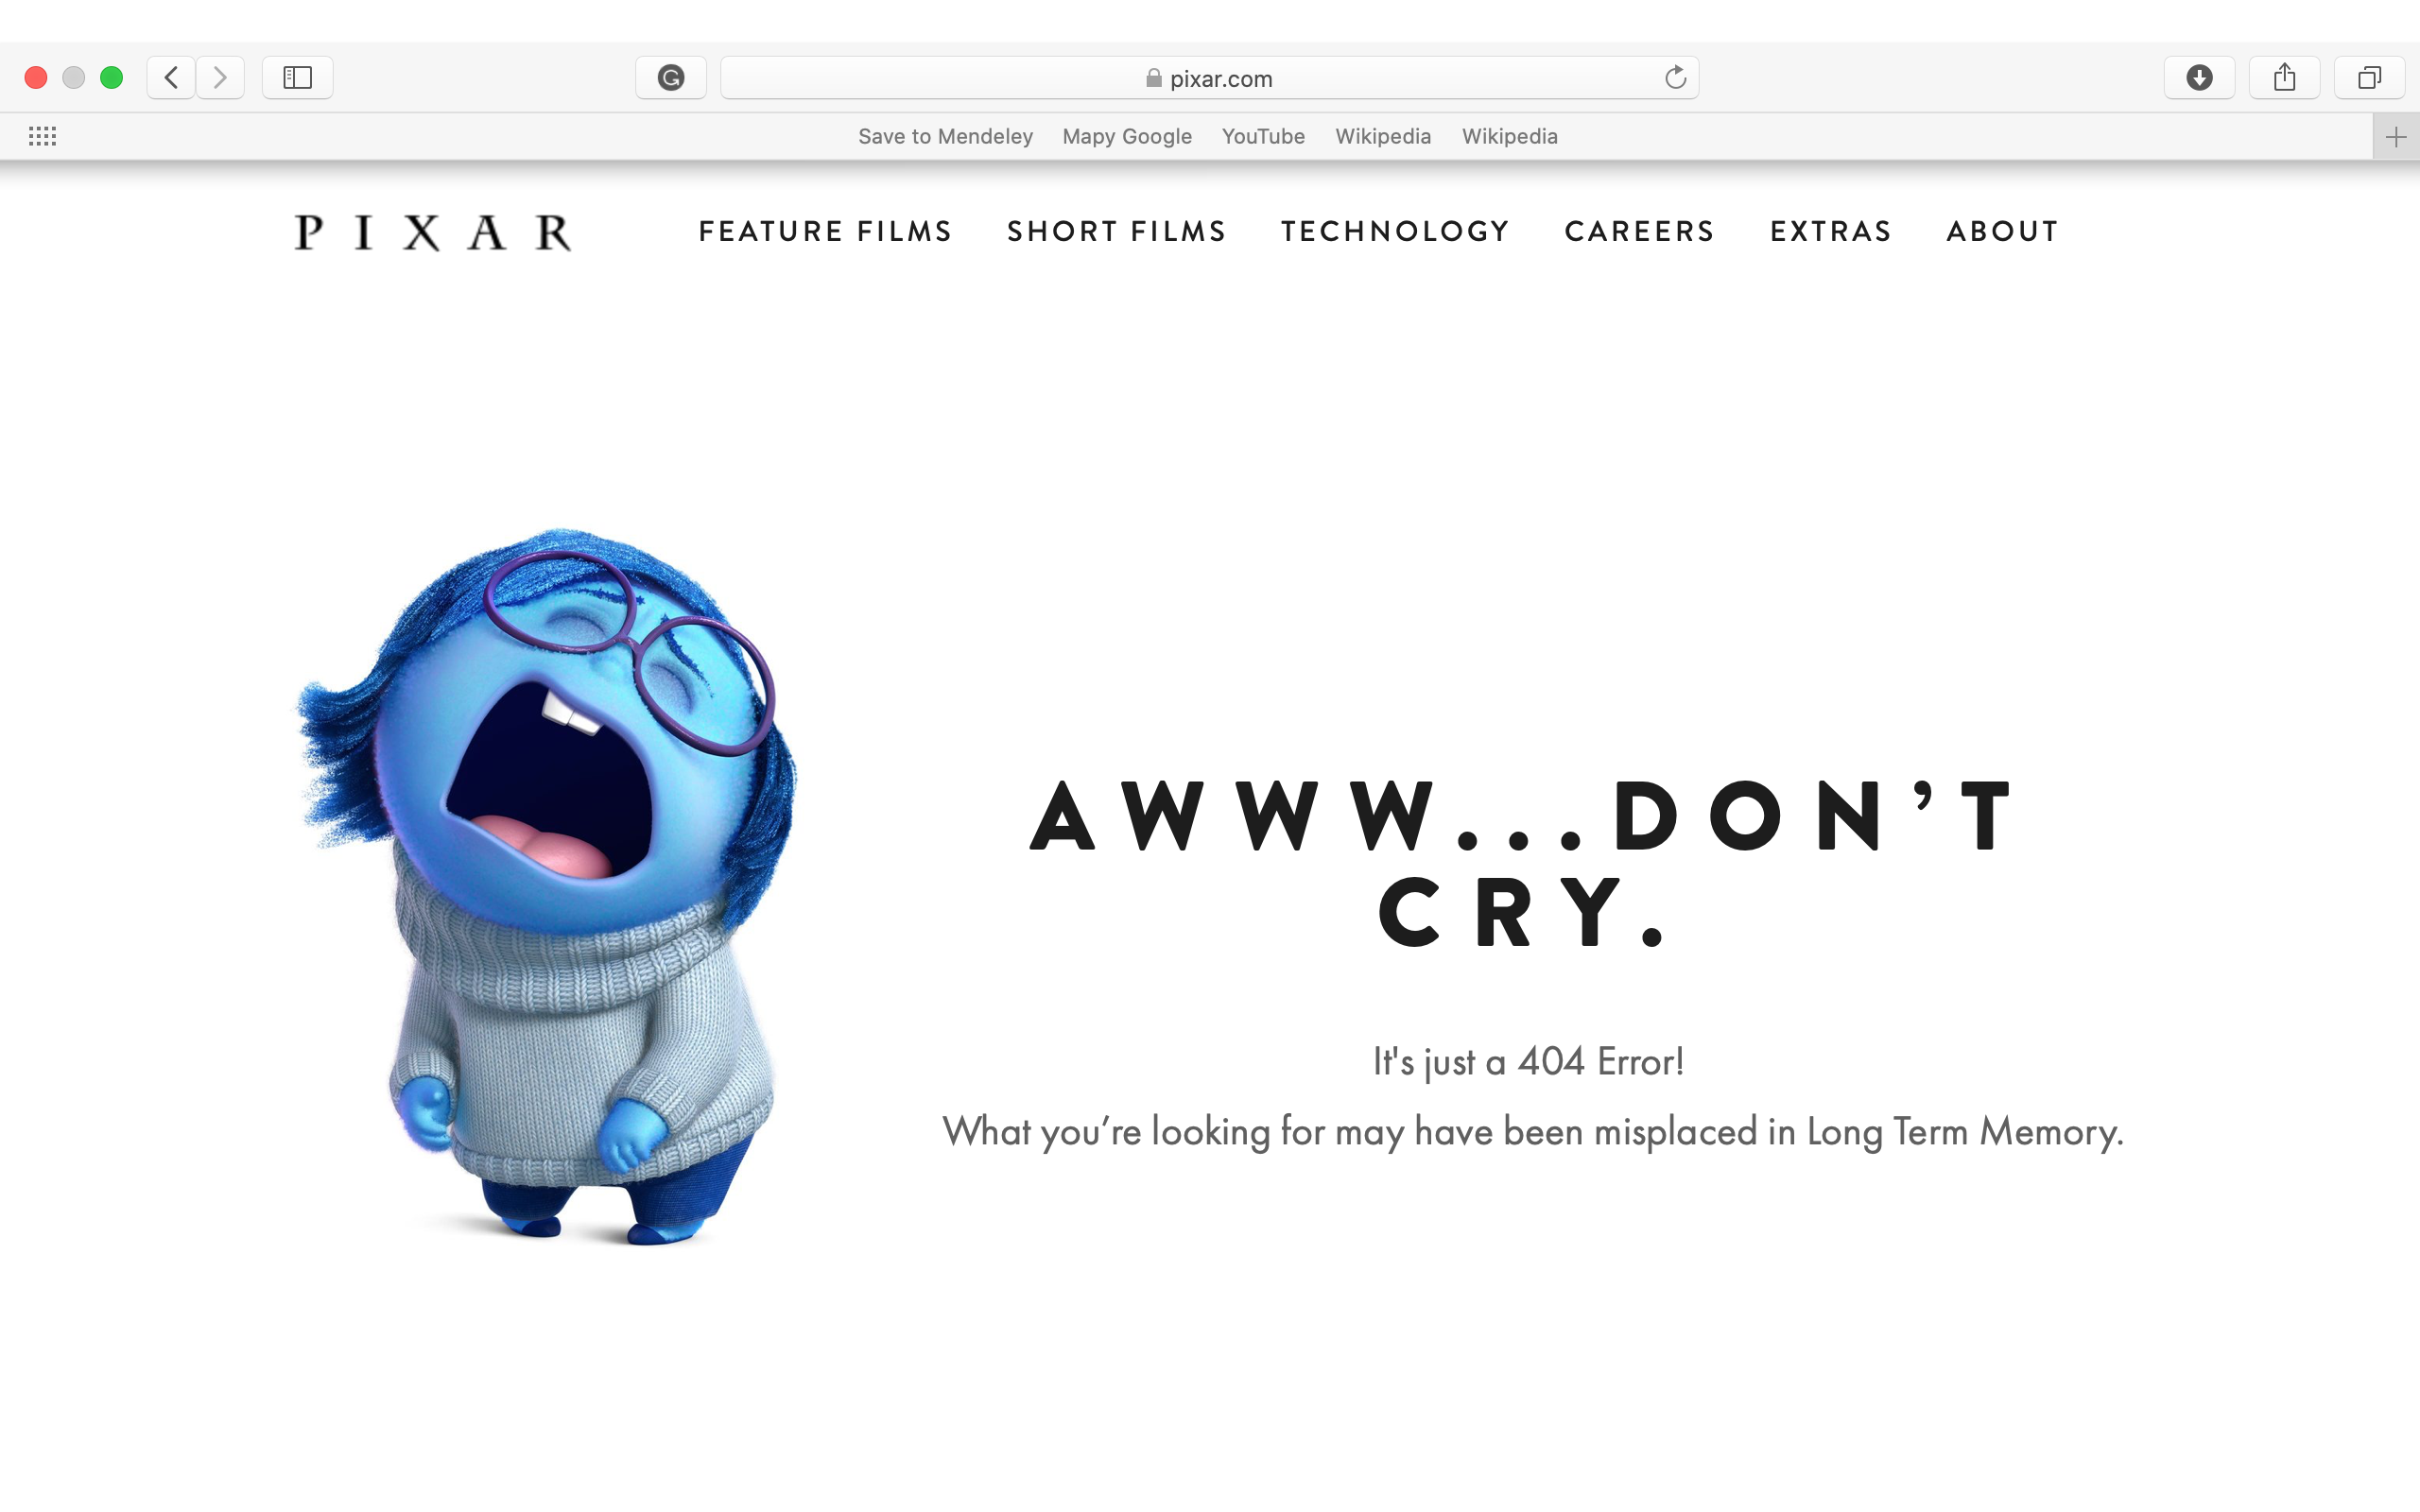
\includegraphics[width = \framewidth]{png/error_404.png}
    }
    \only<+>{
        \frametitle{HTTP Response}
        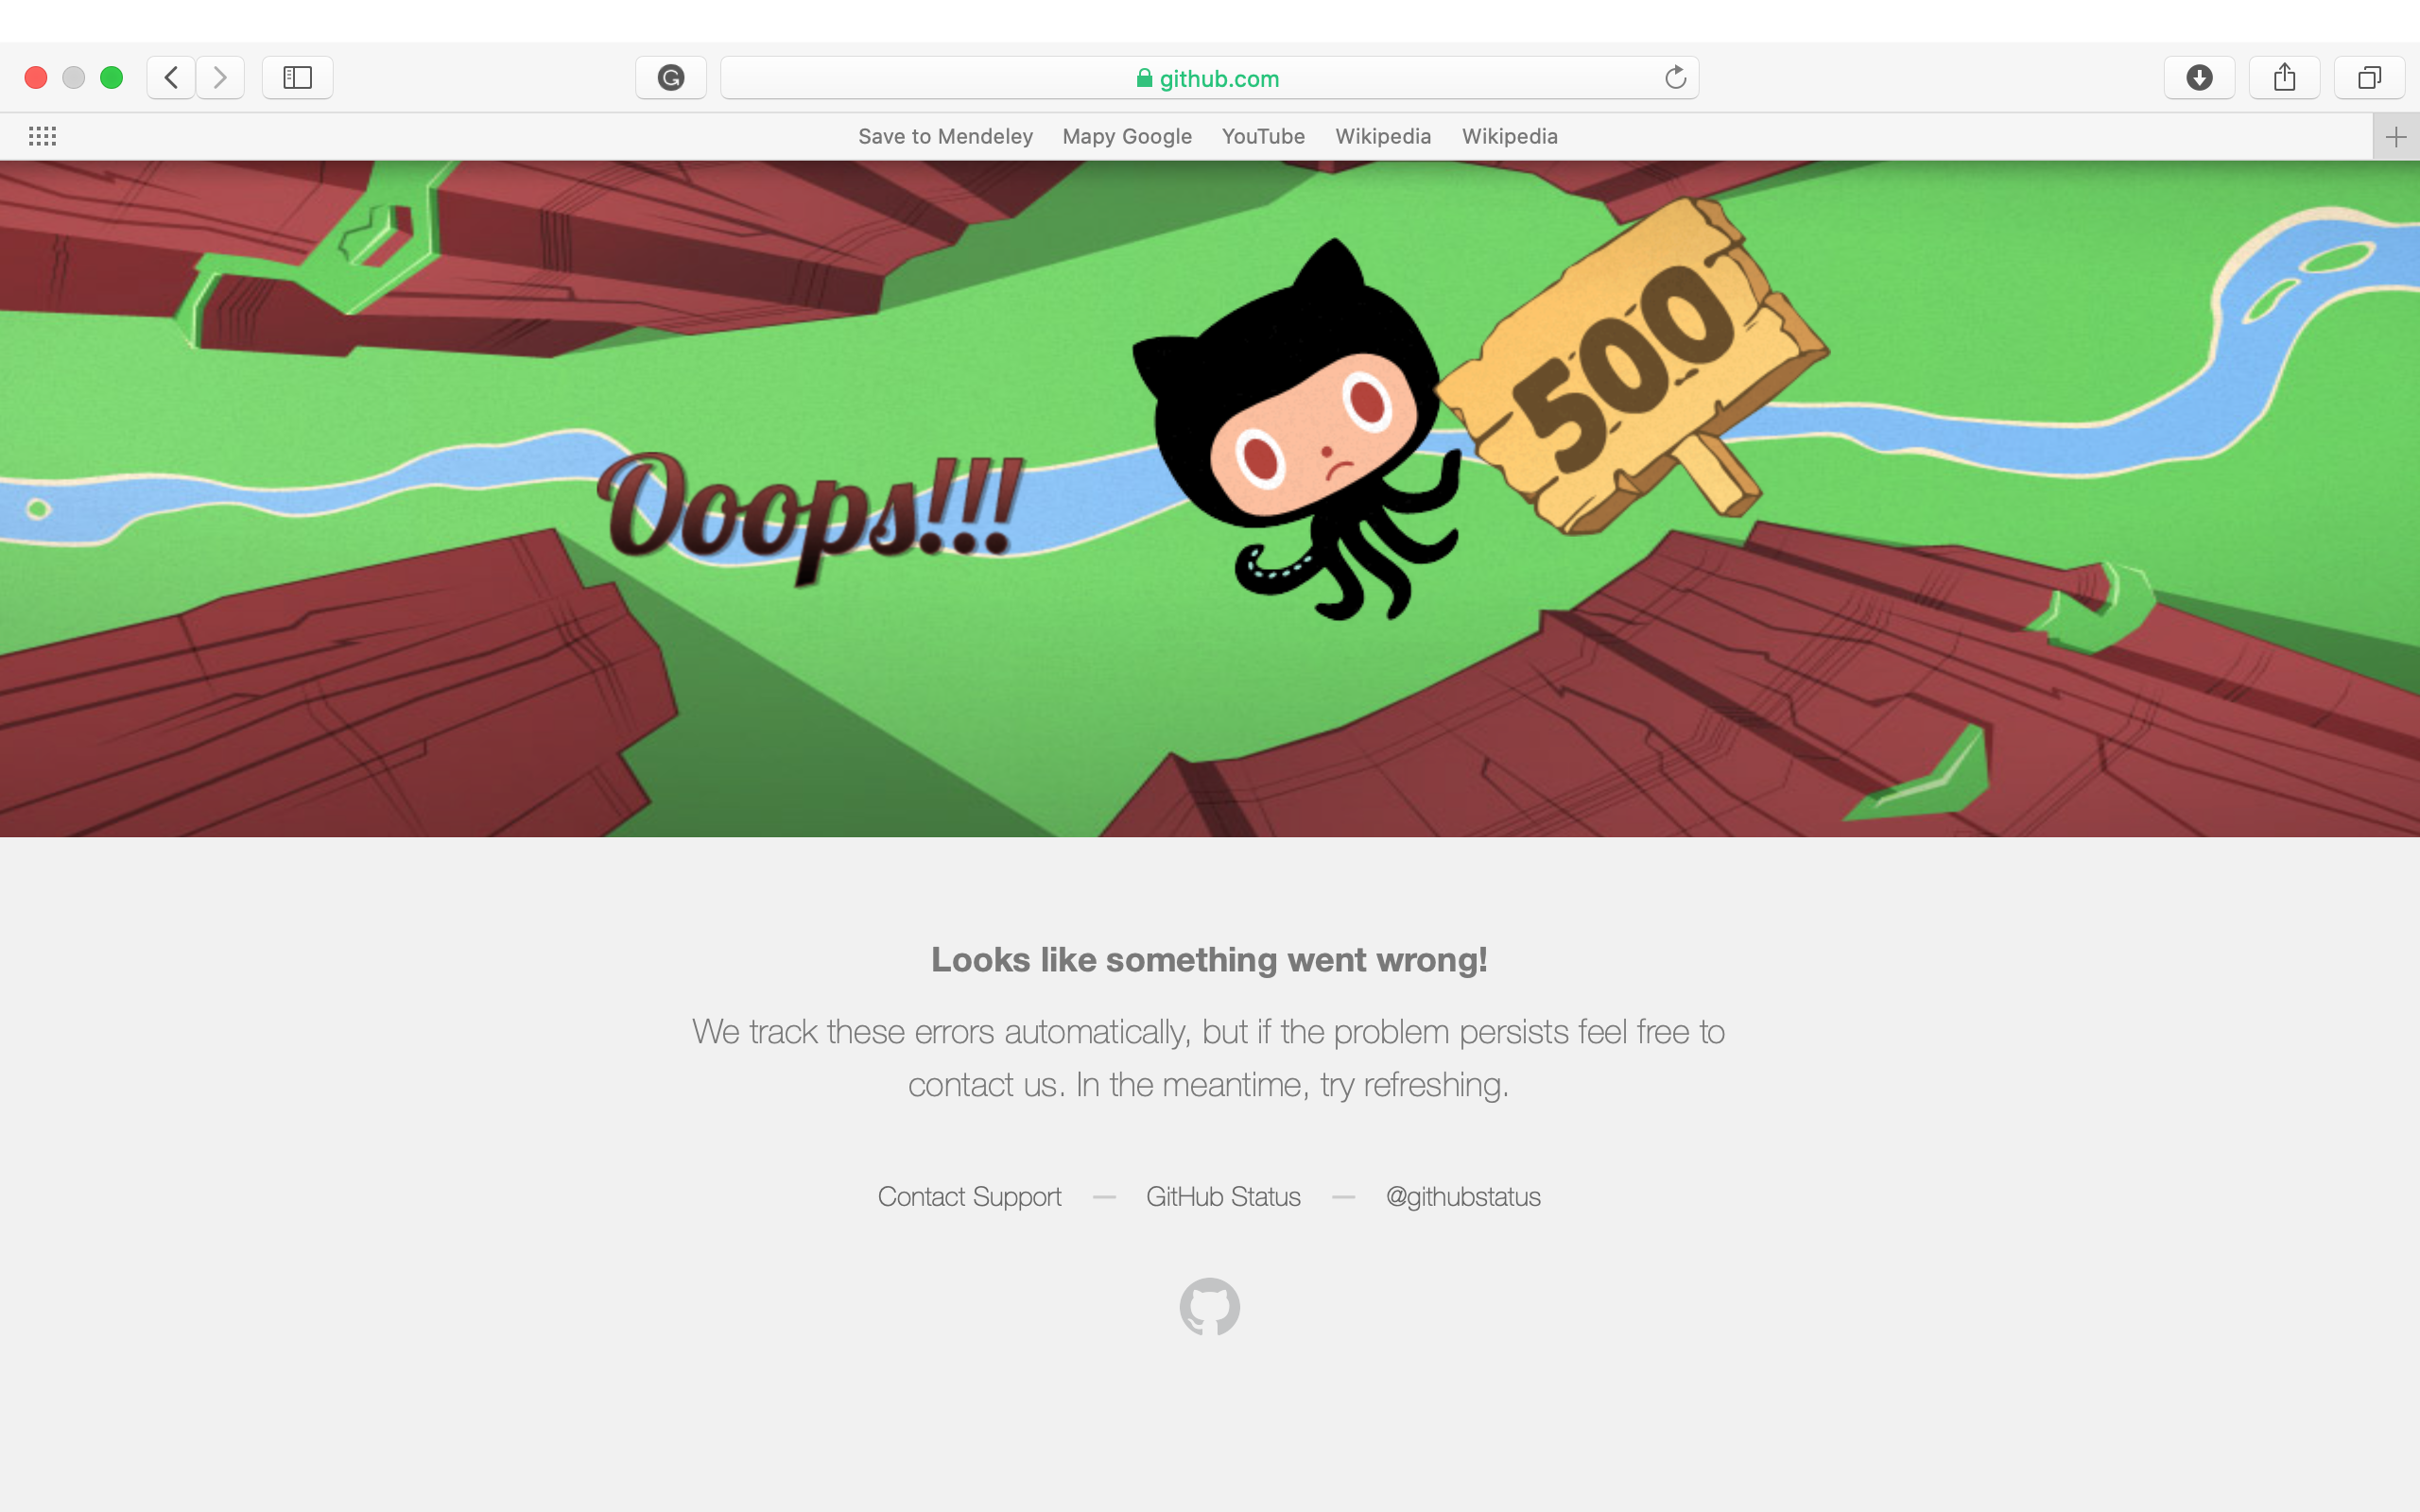
\includegraphics[width = \framewidth]{png/error_500.png}
    }
    \only<+>{
        \frametitle{HTTP Responses}
        HTTP Response is typically composed of:
        \begin{itemize}
            \item A status line (HTTP version, a status code, and a status text)
            \item A set of HTTP headers specifying the response, or describing the body included in the message.
            \item An optional body containing data associated with the response
        \end{itemize}
    }
    \only<+>{
        \frametitle{HTTP Response Status Codes}
        \begin{itemize}
            \item Informational response (100–199);
            \item Successful responses (200–299);
            \item Redirects (300–399);
            \item Client errors (400–499);
            \item Server errors (500–599).
        \end{itemize}
        \blfootnote{Detailed documentation on \textcolor{blue}{\href{https://developer.mozilla.org/en-US/docs/Web/HTTP/Status}{Response Status Codes}}}
    }
\end{frame}

\begin{frame}[fragile]
    \frametitle{HTTP Response}
    \begin{minted}[escapeinside=||,mathescape=true]{html}
    HTTP/1.1 200 OK
    Access-control-allow-methods: GET,HEAD
    Age: 94618
    Content-language: en
    Content-length: 881
    Content-type: application/json
    Date: Wed, 30 Oct 2019 00:18:58 GMT
    Body: {
        "type": "standard",
        "title": "Justyna Kowalczyk",
        "page_id": 4212731,
        "lang": "en",
        "revision": revision,
        "summary": "Justyna Kowalczyk |<|3"
    }
    \end{minted}
\end{frame}

\section{Data formats}

\subsection{JSON}
\begin{frame}[fragile]
    \frametitle{JSON - JavaScript Object Notation}
    \begin{minted}[fontsize=\footnotesize]{js}
    {
        "name": "Alice",
        "age": 17,
        "interests": [
            {
                "name": "physics",
                "disciplines": [
                    "quantum physics",
                    "string theory"
                ]
            },
            {
                "name": "sport",
                "disciplines": [
                    "fishing",
                    "football"
                ]
            }
        ]
    }
    \end{minted}
\end{frame}

\begin{frame}[fragile]
    \frametitle{JSON - JavaScript Object Notation}
    \begin{minted}[fontsize=\footnotesize]{js}
    {
        "name": "Bob",
        "age": 15,
        "interests": [
            {
                "name": "sport",
                "disciplines": [
                    "football"
                ]
            }
        ]
    }
    \end{minted}
    \end{frame}

\begin{frame}
    \frametitle{JSON - JavaScript Object Notation}
    \begin{definition}
        \emph{JavaScript Object Notation} is a lightweight text data format that is relatively easy to read for both the human naked eye and computers. Although it derives from JavaScript it is a language-independent data format. JSON is built on two structures: a collection of key-item pairs and ordered list of values. JSON filenames use .json extension.
    \end{definition}
\end{frame}




